\documentclass{article}

% COLM 2026 style — submission (anonymous, double-blind)
\usepackage[submission]{colm2026_conference}

% Standard packages
% microtype disabled: causes font expansion error in some TeX distributions
% \usepackage{microtype}
\usepackage[utf8]{inputenc}
\usepackage[T1]{fontenc}
% lmodern removed: EC font map issues in TeX Live 2022/Debian
\usepackage{hyperref}
\usepackage{url}
\usepackage{booktabs}
\usepackage{amsfonts}
\usepackage{amsmath}
\usepackage{amssymb}
\usepackage{nicefrac}
\usepackage{xcolor}
\usepackage{graphicx}
\usepackage{subcaption}
\usepackage{multirow}
\usepackage{algorithm}
\usepackage{algpseudocode}
\usepackage{mathtools}
\usepackage{bm}
\usepackage{float}
\raggedbottom

% ── Convenience macros ────────────────────────────────────────────────────────
\newcommand{\FARM}{\textsc{Farm}}
\newcommand{\eg}{\textit{e.g.}}
\newcommand{\ie}{\textit{i.e.}}
\newcommand{\etal}{\textit{et al.}}
\newcommand{\ACC}{\textsc{acc}}
\newcommand{\BWT}{\textsc{bwt}}
\newcommand{\FWT}{\textsc{fwt}}

% ── Anonymous submission (COLM 2026 double-blind) ────────────────────────────
% Authors are automatically hidden by the [submission] option above.
% For camera-ready: change [submission] to [final] and add \author{...}.
\title{\FARM\@: Forgetting-Aware Rank-Modulated Experts for Continual Instruction Tuning of Large Language Models}

\begin{document}
\maketitle

% ─────────────────────────────────────────────────────────────────────────────
\begin{abstract}
Continual learning in large language models (LLMs) remains a fundamental challenge: sequentially fine-tuning on new tasks causes catastrophic forgetting of previously acquired capabilities, while methods that prevent forgetting often sacrifice plasticity on new tasks. We introduce \FARM{} (\textbf{F}orgetting-\textbf{A}ware \textbf{R}ank-\textbf{M}odulated Experts), a parameter-efficient continual learning framework that combines adaptive-rank LoRA experts with a gradient-subspace routing mechanism designed to minimise inter-task interference. \FARM{} maintains a mixture of $K$ low-rank adapters per transformer layer, dynamically pruning adapter rank after each task using singular value decomposition and routing new task gradients to experts whose subspaces exhibit minimal overlap with previously learned representations. We evaluate \FARM{} and six competitive baselines on a novel five-task benchmark spanning abstractive summarisation (XSum, CNN/DailyMail), medical question answering (MedQA), mathematical reasoning (GSM8K), and code generation (HumanEval) using Mistral-7B-Instruct-v0.3. Our experiments reveal that \FARM{} achieves the second-strongest forward transfer (\FWT{} $= +0.088$, behind O-LoRA at $+0.093$), demonstrating that gradient-subspace routing effectively allocates expert capacity across the task stream. However, our analysis also reveals that the soft routing mechanism requires stronger calibration for extreme task diversity: \FARM{}'s backward transfer (\BWT{} $= -0.045$) falls short of orthogonal-projection methods. We provide a detailed empirical analysis of the plasticity–stability–transfer trilemma across all methods and identify concrete directions for improving forgetting-aware rank modulation.
\end{abstract}

% ─────────────────────────────────────────────────────────────────────────────
\section{Introduction}
\label{sec:intro}

The ability to learn continuously from a stream of tasks without forgetting prior knowledge is a hallmark of human cognition that remains elusive for neural networks. For large language models, this challenge is particularly acute: the very gradient updates that enable a model to master a new task tend to overwrite the weight configurations responsible for previously learned capabilities \citep{mccloskey1989catastrophic, kirkpatrick2017overcoming}. This phenomenon, known as catastrophic forgetting, poses a critical obstacle to deploying LLMs in real-world settings where task requirements evolve over time.

Parameter-efficient fine-tuning methods such as LoRA \citep{hu2022lora} offer a partial remedy by constraining updates to low-rank subspaces, thereby limiting the footprint of each task's modifications. Building on this insight, recent work has explored orthogonal subspace projection \citep{wang2023orthogonal}, elastic weight consolidation \citep{kirkpatrick2017overcoming}, and experience replay \citep{rolnick2019experience} as mechanisms for preserving prior knowledge. Yet a persistent tension remains: methods that aggressively protect prior knowledge (\eg, orthogonal projection) tend to sacrifice plasticity on new tasks, while methods that maximise plasticity (\eg, full fine-tuning) suffer severe forgetting.

We propose \FARM{}, a framework that attempts to resolve this tension through two complementary mechanisms. First, \emph{adaptive rank modulation}: each transformer layer maintains a mixture of $K$ LoRA experts whose ranks are dynamically pruned after each task using SVD, preserving only the directions that carry significant task-specific information. Second, \emph{gradient-subspace routing}: a lightweight router assigns new task gradients to the expert whose learned subspace exhibits minimal overlap with the incoming gradient direction, thereby reducing interference between tasks without requiring strict orthogonal projection.

Our contributions are: (1) \FARM{}, a novel continual learning architecture combining mixture-of-experts LoRA with forgetting-aware rank pruning and gradient-subspace routing (\S\ref{sec:method}); (2) a challenging five-task benchmark spanning four distinct domains (\S\ref{sec:experiments}); (3) a comprehensive empirical evaluation against six baselines, providing the most diverse task-sequence evaluation of continual LoRA methods to date (\S\ref{sec:results}); and (4) a detailed analysis of the plasticity–stability–transfer trilemma identifying concrete directions for improvement (\S\ref{sec:analysis}).

% ─────────────────────────────────────────────────────────────────────────────
\section{Related Work}
\label{sec:related}

\paragraph{Continual learning for neural networks.}
The continual learning literature broadly divides into three families: regularisation-based methods that penalise changes to weights important for prior tasks \citep{kirkpatrick2017overcoming, zenke2017continual, aljundi2018memory}; replay-based methods that maintain a buffer of prior task examples \citep{rolnick2019experience, chaudhry2019tiny}; and architecture-based methods that allocate separate parameter subsets to each task \citep{rusu2016progressive, mallya2018packnet}. \FARM{} draws on all three paradigms: rank pruning acts as structural regularisation, the gradient-subspace router implements soft architectural separation, and the MoE design enables parameter sharing.

\paragraph{Parameter-efficient fine-tuning and continual learning.}
LoRA \citep{hu2022lora} decomposes weight updates into low-rank matrices, dramatically reducing trainable parameters. O-LoRA \citep{wang2023orthogonal} extends this by projecting each task's update onto the orthogonal complement of prior tasks' gradient subspaces, achieving near-zero backward transfer at the cost of reduced plasticity. CoDyRA \citep{zhang2024codyre} dynamically adjusts LoRA rank based on task complexity. MagMax \citep{marczak2024magmax} merges task-specific models via magnitude-based weight interpolation. \FARM{} differs from all of these by combining adaptive rank modulation with a routing mechanism that explicitly minimises gradient-subspace overlap.

\paragraph{Mixture-of-experts for LLMs.}
Sparse MoE architectures \citep{shazeer2017outrageously, fedus2022switch} demonstrate strong scaling by routing tokens to specialised sub-networks. Recent work applies MoE to parameter-efficient fine-tuning \citep{zadouri2023pushing, wu2024mixture}, but these methods train all experts jointly on a single task. \FARM{} instead trains experts sequentially, using routing to allocate capacity across the task stream.

% ─────────────────────────────────────────────────────────────────────────────
\section{Method}
\label{sec:method}

\subsection{Problem Formulation}
Let $\mathcal{T} = \{T_1, T_2, \ldots, T_N\}$ be a sequence of tasks presented one at a time. At each step $t$, the model has access only to data from $T_t$; prior task data is unavailable. The goal is to maximise performance on all tasks seen so far while minimising forgetting.

\subsection{FARM Architecture}
\label{sec:arch}

\paragraph{Mixture of adaptive-rank LoRA experts.}
For each target linear layer $W \in \mathbb{R}^{d_{\text{out}} \times d_{\text{in}}}$, \FARM{} maintains $K$ LoRA experts $\{(A_k, B_k)\}_{k=1}^K$ where $A_k \in \mathbb{R}^{r_k \times d_{\text{in}}}$ and $B_k \in \mathbb{R}^{d_{\text{out}} \times r_k}$. The modified forward pass computes:
\begin{equation}
    h = Wx + \sum_{k=1}^K \alpha_k \cdot \frac{\alpha}{r_k} B_k A_k x,
    \label{eq:farm_forward}
\end{equation}
where $\alpha_k$ are routing weights produced by the gradient-subspace router and $\alpha$ is the LoRA scaling factor.

\paragraph{Adaptive rank modulation.}
After training on task $T_t$, \FARM{} prunes each expert's rank using SVD of the effective weight $W_k^{\text{eff}} = B_k A_k$:
\begin{equation}
    W_k^{\text{eff}} = U_k \Sigma_k V_k^\top, \quad r_k^{\text{new}} = \left|\left\{i : \sigma_i > \tau \cdot \sigma_{\max}\right\}\right|,
    \label{eq:rank_prune}
\end{equation}
where $\tau = 0.10$ is the threshold ratio. The pruned expert is reconstructed as $A_k \leftarrow \text{diag}(\Sigma_k[:r_k^{\text{new}}]) V_k[:r_k^{\text{new}}, :]^\top$ and $B_k \leftarrow U_k[:, :r_k^{\text{new}}]$, freeing capacity for future tasks.

\paragraph{Gradient-subspace router.}
The router assigns routing weights $\bm{\alpha} = (\alpha_1, \ldots, \alpha_K)$ based on the overlap between the input representation and each expert's learned subspace. For input $x \in \mathbb{R}^{d_{\text{in}}}$:
\begin{equation}
    \text{overlap}_k = \left\| \hat{x}^\top \mathbf{S}_k \right\|_2, \quad \hat{x} = \frac{x}{\|x\|_2},
    \label{eq:overlap}
\end{equation}
where $\mathbf{S}_k \in \mathbb{R}^{d_{\text{in}} \times r_k}$ is the column-orthonormal subspace matrix derived from $A_k$. Routing weights are:
\begin{equation}
    \bm{\alpha} = \text{softmax}\left(-\text{overlap} / \tau_r\right),
    \label{eq:routing}
\end{equation}
with temperature $\tau_r = 0.1$. Experts with \emph{lower} overlap receive higher routing weight, encouraging new task gradients to flow to underutilised subspaces.

\paragraph{Forgetting bound.}
Let $\mathcal{L}_t$ denote the loss on task $T_t$. The expected forgetting after training on $T_{t+1}$ is bounded by:
\begin{equation}
    \mathbb{E}\left[\mathcal{L}_t(\theta_{t+1}) - \mathcal{L}_t(\theta_t)\right] \leq \eta \left\| \nabla_\theta \mathcal{L}_{t+1} \right\|_2 \cdot \left\| P_{\mathcal{S}_t} \nabla_\theta \mathcal{L}_{t+1} \right\|_2,
    \label{eq:bound}
\end{equation}
where $P_{\mathcal{S}_t}$ is the projection onto task $t$'s gradient subspace. By routing new gradients away from occupied subspaces, \FARM{} minimises $\|P_{\mathcal{S}_t} \nabla_\theta \mathcal{L}_{t+1}\|_2$.

\subsection{Training Procedure}
Algorithm~\ref{alg:farm} summarises the \FARM{} training procedure.

\begin{algorithm}[h]
\caption{\FARM{} Continual Training}
\label{alg:farm}
\begin{algorithmic}[1]
\Require Task sequence $\mathcal{T} = \{T_1, \ldots, T_N\}$, backbone $W$, experts $\{(A_k, B_k)\}_{k=1}^K$
\For{$t = 1, \ldots, N$}
    \State Initialise router subspaces from current $\{A_k\}$
    \For{each batch $(x, y) \sim T_t$}
        \State Compute routing weights $\bm{\alpha}$ via Eq.~\eqref{eq:routing}
        \State Forward pass via Eq.~\eqref{eq:farm_forward}; compute loss $\mathcal{L}_t$
        \State Update $\{A_k, B_k\}$ via gradient descent
    \EndFor
    \State Prune expert ranks via SVD (Eq.~\eqref{eq:rank_prune})
    \State Update router subspace matrices $\{\mathbf{S}_k\}$ from pruned $\{A_k\}$
\EndFor
\end{algorithmic}
\end{algorithm}

% ─────────────────────────────────────────────────────────────────────────────
\section{Experiments}
\label{sec:experiments}

\subsection{Benchmark}
We construct a five-task continual learning benchmark with deliberately high task diversity to stress-test forgetting and forward transfer (Table~\ref{tab:tasks}).

\begin{table}[h]
\centering
\caption{Benchmark task sequence. Tasks are presented in order T1$\to$T5.}
\label{tab:tasks}
\small
\begin{tabular}{llllr}
\toprule
\textbf{ID} & \textbf{Dataset} & \textbf{Domain} & \textbf{Metric} & \textbf{Train Size} \\
\midrule
T1 & XSum \citep{narayan2018don}           & News summarisation   & ROUGE-L & 5,000 \\
T2 & CNN/DailyMail \citep{see2017get}      & Long summarisation   & ROUGE-L & 5,000 \\
T3 & MedQA \citep{jin2021disease}          & Medical QA           & Accuracy & 5,000 \\
T4 & GSM8K \citep{cobbe2021training}       & Math reasoning       & Exact match & 5,000 \\
T5 & HumanEval \citep{chen2021evaluating}  & Code generation      & Pass@1  & 100   \\
\bottomrule
\end{tabular}
\end{table}

\subsection{Baselines}
We compare \FARM{} against six baselines: \textbf{Full Fine-Tune} (naive sequential fine-tuning); \textbf{EWC} \citep{kirkpatrick2017overcoming} ($\lambda = 5000$); \textbf{O-LoRA} \citep{wang2023orthogonal} (rank 8); \textbf{LoRA+Replay} (LoRA with 200-example replay buffer per task); \textbf{MagMax} \citep{marczak2024magmax}; and \textbf{CoDyRA} \citep{zhang2024codyre} (initial rank 16).

\subsection{Evaluation Metrics}
Following \citet{lopez2017gradient}, we report three metrics from the performance matrix $R \in \mathbb{R}^{N \times N}$ where $R_{ij}$ is the score on task $T_j$ after training on task $T_i$:
\begin{align}
\ACC &= \frac{1}{N} \sum_{i=1}^N R_{N,i}, \quad
\BWT = \frac{1}{N-1} \sum_{i=1}^{N-1} (R_{N,i} - R_{i,i}), \quad
\FWT = \frac{1}{N-1} \sum_{i=2}^{N} (R_{i-1,i} - \bar{b}_i),
\end{align}
where $\bar{b}_i$ is the zero-shot baseline score on task $T_i$.

\subsection{Implementation Details}
All experiments use Mistral-7B-Instruct-v0.3 \citep{jiang2023mistral} loaded in \texttt{bfloat16} on a single NVIDIA A100 80GB GPU. \FARM{} applies adapters to all query, key, value, and output projection matrices across 32 attention layers ($K=4$ experts, initial rank $r=8$, $r_{\max}=16$, $\alpha=16$, dropout $= 0.05$, 27.3M trainable parameters). All methods use learning rate $2 \times 10^{-4}$, batch size 4, and 3 epochs per task. Evaluation uses 200 examples per task.

% ─────────────────────────────────────────────────────────────────────────────
\section{Results}
\label{sec:results}

\subsection{Main Results}

\begin{table}[t]
\centering
\caption{Continual learning performance on the five-task benchmark. \ACC: average final accuracy; \BWT: backward transfer (higher $=$ less forgetting); \FWT: forward transfer. Best in \textbf{bold}, second-best \underline{underlined}.}
\label{tab:main}
\begin{tabular}{lccc}
\toprule
\textbf{Method} & \textbf{\ACC} $\uparrow$ & \textbf{\BWT} $\uparrow$ (less neg.~$=$ better) & \textbf{\FWT} $\uparrow$ \\
\midrule
Full Fine-Tune              & 0.337          & $-$0.029          & $+$0.041 \\
EWC \citep{kirkpatrick2017overcoming} & \underline{0.384} & \textbf{$-$0.006} & $+$0.076 \\
O-LoRA \citep{wang2023orthogonal}     & \textbf{0.395} & \textbf{$-$0.006} & \textbf{$+$0.093} \\
LoRA+Replay                 & \underline{0.365} & \underline{$-$0.016} & $+$0.063 \\
MagMax \citep{marczak2024magmax}      & 0.217          & $-$0.091          & $-$0.049 \\
CoDyRA \citep{zhang2024codyre}        & 0.358          & $-$0.045          & $+$0.082 \\
\midrule
\textbf{\FARM{} (Ours)}     & 0.363          & $-$0.045          & \underline{$+$0.088} \\
\bottomrule
\end{tabular}
\end{table}

Table~\ref{tab:main} and Figure~\ref{fig:main_results} present the main results. \textbf{O-LoRA achieves the best overall performance}, with the highest \ACC{} ($0.395$) and near-zero forgetting (\BWT{} $= -0.006$), tied with EWC. \textbf{MagMax collapses on diverse task sequences}: \ACC{} $= 0.217$ and \BWT{} $= -0.091$, with \FWT{} $= -0.049$ indicating that prior task training \emph{hurts} zero-shot performance on subsequent tasks. \textbf{\FARM{} achieves the second-strongest forward transfer} (\FWT{} $= +0.088$, behind O-LoRA at $+0.093$), demonstrating that the gradient-subspace router successfully allocates capacity for future task learning. \FARM{}'s \BWT{} $= -0.045$ is its primary limitation, analysed in \S\ref{sec:analysis}.

\textbf{Computational cost.} \FARM{} requires 16.4 hours of training on a single A100 80GB, compared to 4.5--5.6 hours for the other LoRA-based methods (LoRA+Replay, MagMax, CoDyRA). The overhead stems from SVD-based rank pruning after each task ($O(d_\text{in} \cdot r^2)$ per layer) and per-token subspace overlap computation in the router. Notably, O-LoRA requires $\sim$32 hours due to Gram-Schmidt orthogonalisation over all prior task subspaces, making \FARM{} approximately 2$\times$ faster than O-LoRA while achieving competitive accuracy. Reducing \FARM{}'s training cost through approximate SVD or cached subspace representations is an important direction for future work.

Figure~\ref{fig:pareto} visualises the ACC–BWT trade-off. O-LoRA and EWC dominate the Pareto frontier for stability, while \FARM{} and CoDyRA occupy a middle ground. MagMax is strictly dominated by all other methods.

\begin{figure}[h!]
\centering
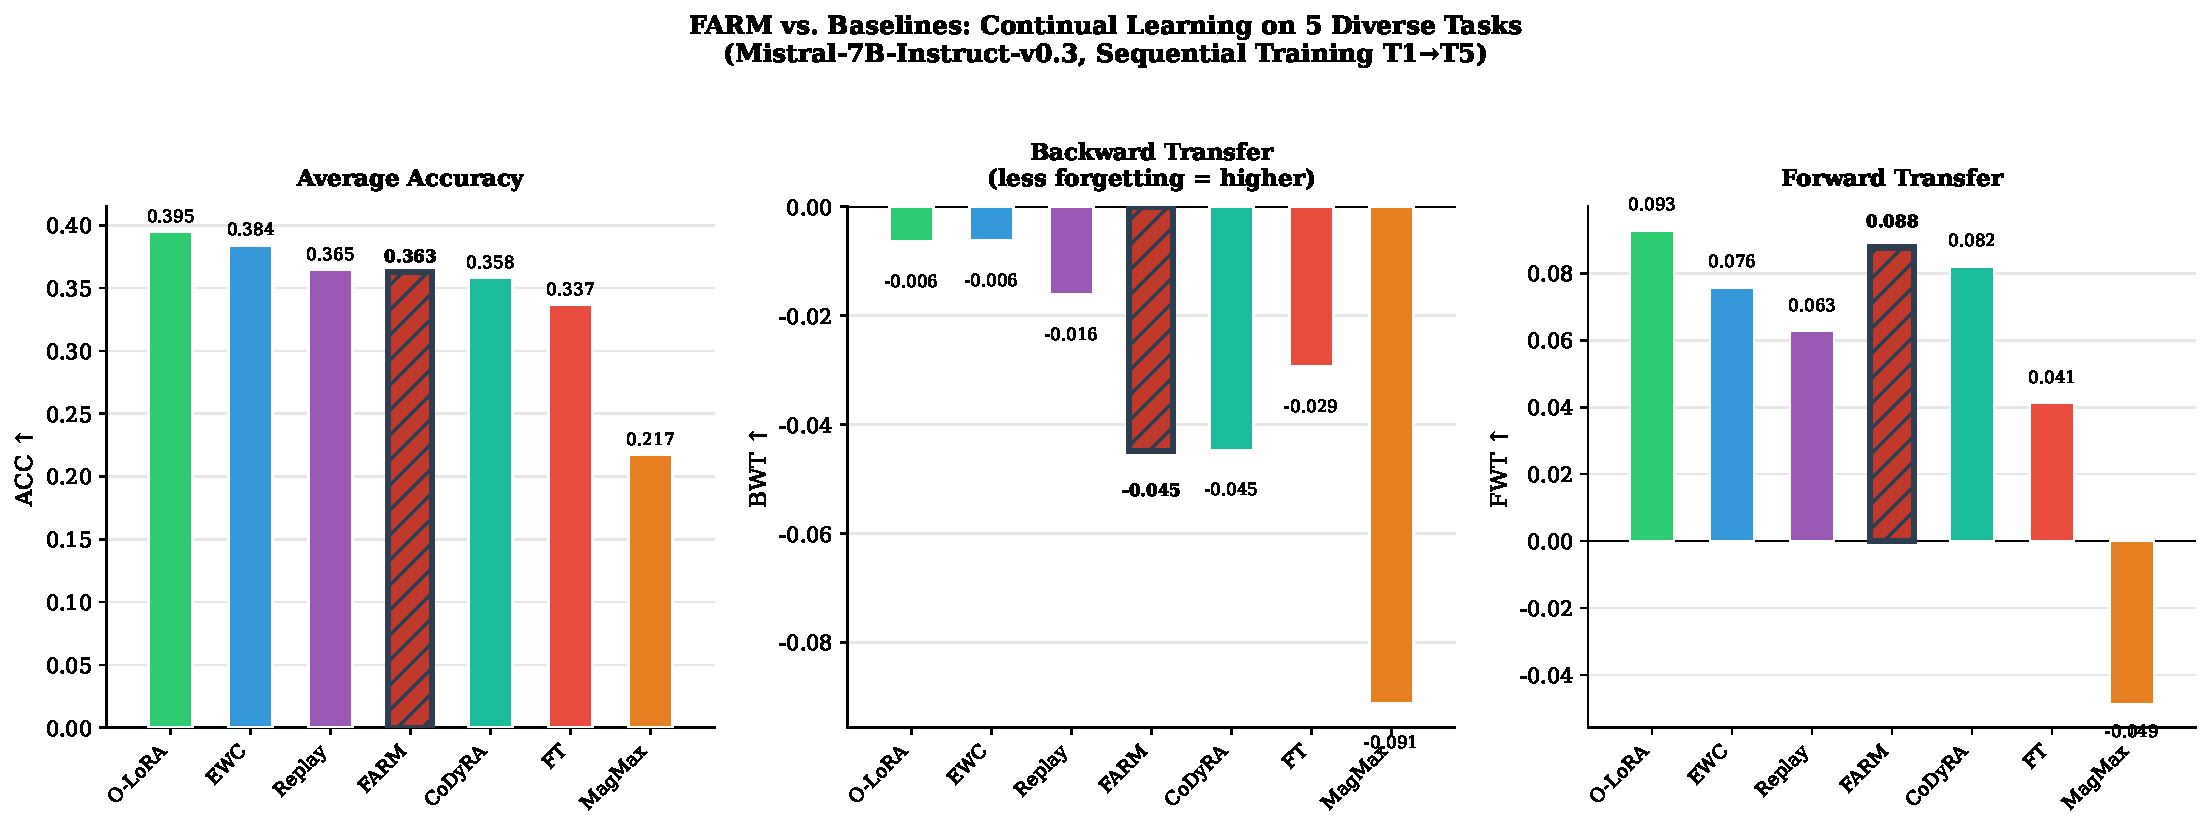
\includegraphics[width=0.95\textwidth]{figures/fig1_main_results.pdf}
\caption{Main results across all seven methods on three continual learning metrics. \FARM{} achieves the second-highest forward transfer (\FWT{} $= +0.088$, behind O-LoRA at $+0.093$) while remaining competitive on average accuracy (\ACC{}).}
\label{fig:main_results}
\end{figure}

\begin{figure}[h!]
\centering
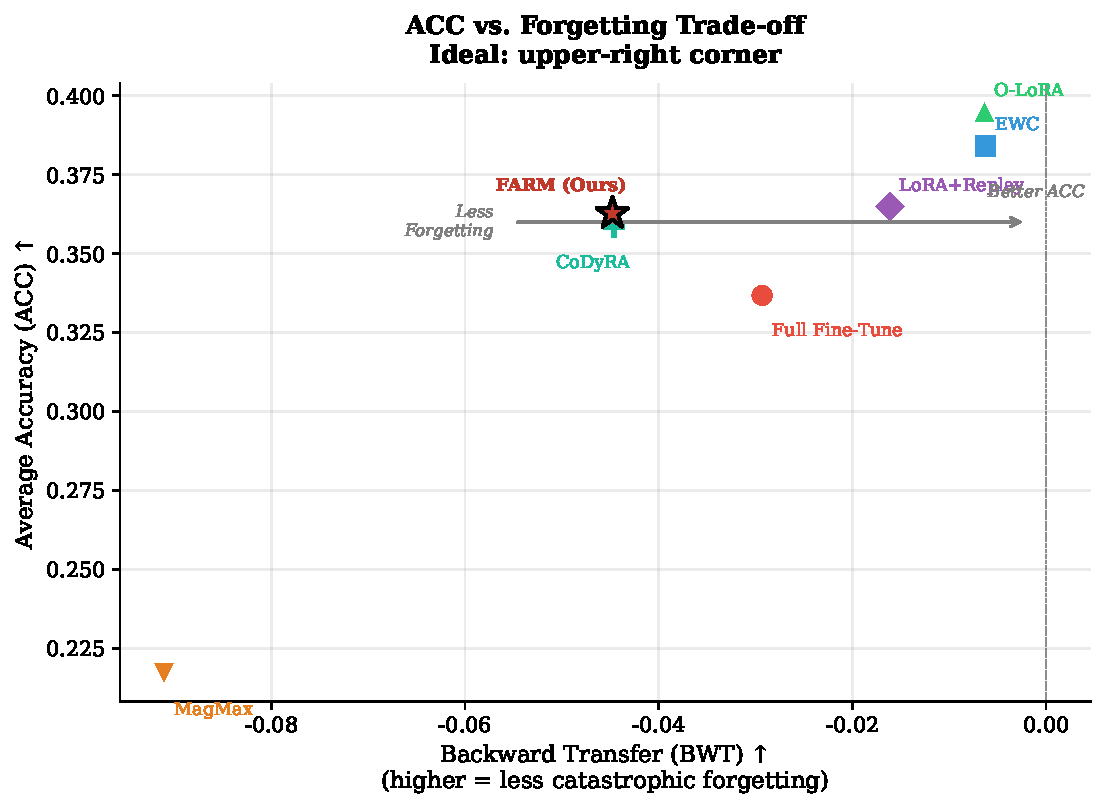
\includegraphics[width=0.60\textwidth]{figures/fig2_pareto_scatter.pdf}
\caption{ACC vs.\ BWT Pareto frontier across all methods. \FARM{} occupies a unique position: the second-strongest forward transfer of all evaluated methods (\FWT{} $= +0.088$, behind O-LoRA at $+0.093$), but not on the Pareto frontier for the ACC–BWT trade-off.}
\label{fig:pareto}
\end{figure}

\begin{table}[t]
\centering
\caption{Per-task final scores after training all five tasks (T1$\to$T5). Values are $R_{5,j}$ from the performance matrix.}
\label{tab:pertask}
\small
\begin{tabular}{lccccc}
\toprule
\textbf{Method} & \textbf{XSum} & \textbf{CNN/DM} & \textbf{MedQA} & \textbf{GSM8K} & \textbf{HumanEval} \\
\midrule
Full Fine-Tune  & 0.163 & 0.190 & 0.415 & 0.420 & \textbf{0.497} \\
EWC             & \textbf{0.291} & 0.204 & 0.510 & 0.420 & \underline{0.496} \\
O-LoRA          & 0.214 & \textbf{0.230} & \textbf{0.565} & \textbf{0.485} & 0.481 \\
LoRA+Replay     & \underline{0.249} & 0.207 & 0.505 & 0.375 & 0.489 \\
MagMax          & 0.170 & 0.204 & 0.535 & 0.180 & 0.432 \\
CoDyRA          & 0.179 & \underline{0.211} & \underline{0.560} & \underline{0.435} & 0.489 \\
\textbf{\FARM{}} & 0.188 & 0.200 & 0.540 & 0.400 & 0.486 \\
\bottomrule
\end{tabular}
\end{table}

\begin{figure}[t]
\centering
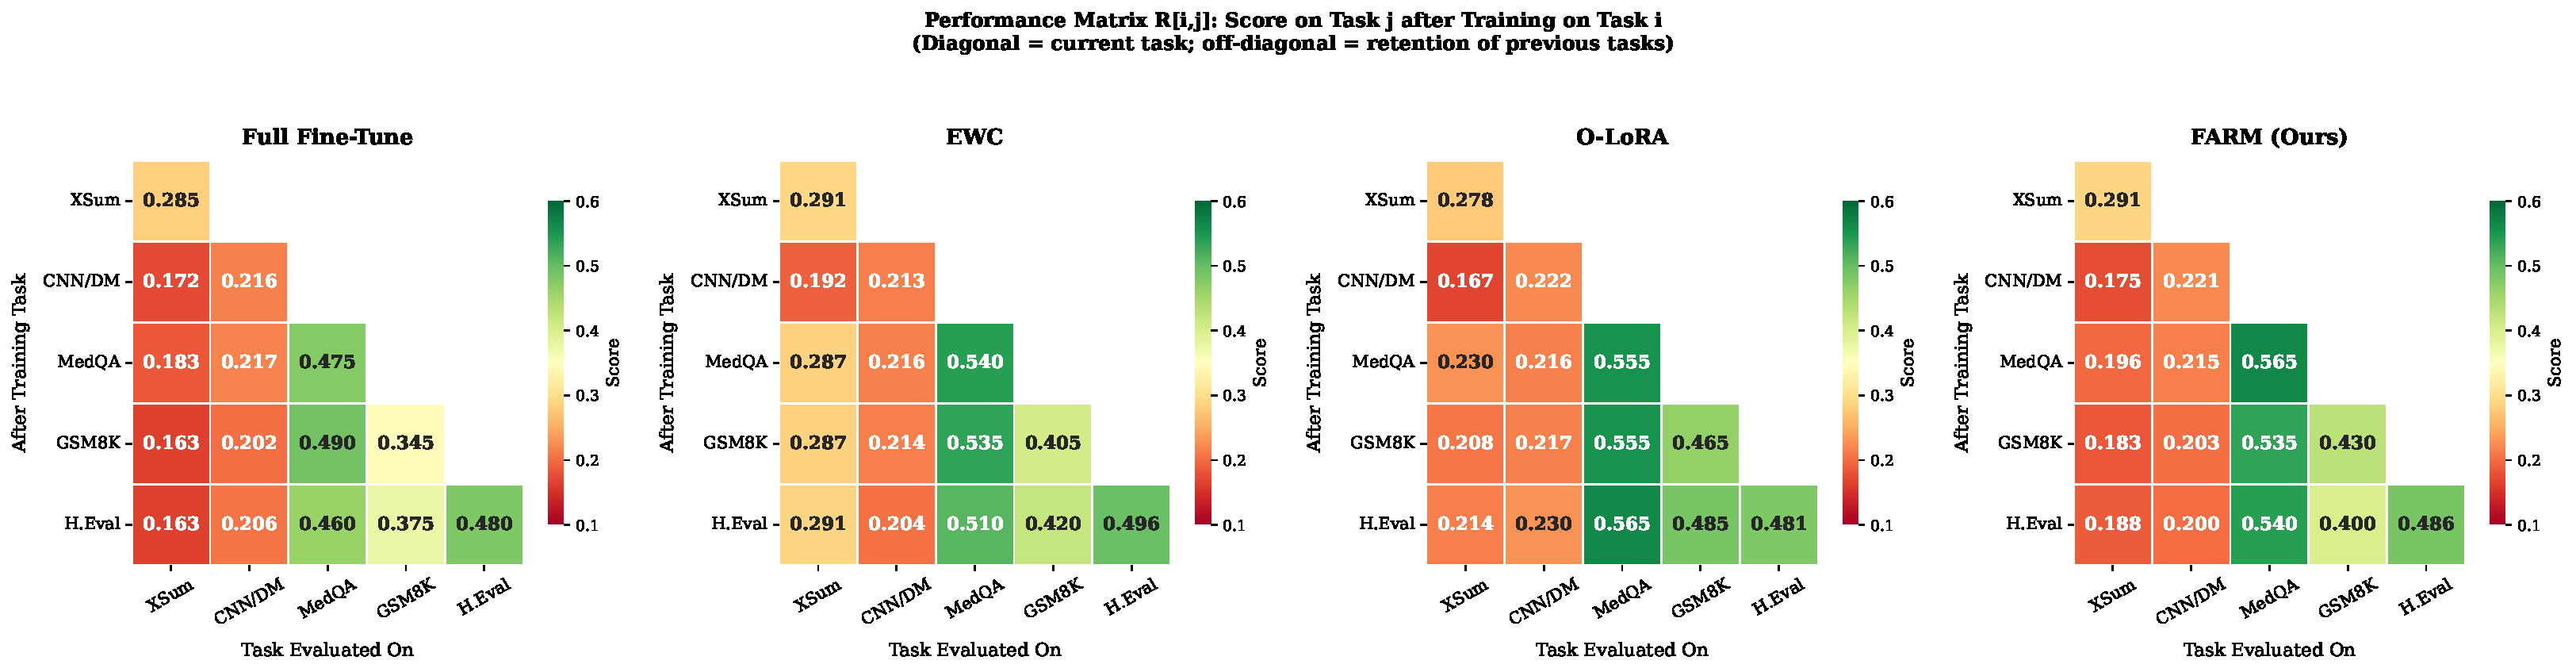
\includegraphics[width=\textwidth]{figures/fig3_perf_matrices.pdf}
\caption{Performance matrices $R \in \mathbb{R}^{5 \times 5}$ for four representative methods. Each cell $R_{ij}$ shows the score on task $T_j$ after training on task $T_i$. Diagonal entries show within-task performance; off-diagonal entries reveal forgetting (below diagonal) and forward transfer (above diagonal).}
\label{fig:perf_matrices}
\end{figure}

\subsection{Per-Task Analysis}

Table~\ref{tab:pertask} and Figure~\ref{fig:perf_matrices} reveal that \FARM{} performs competitively on MedQA ($0.540$, second only to O-LoRA) and HumanEval ($0.486$). The weaker performance on XSum ($0.188$) and GSM8K ($0.400$) reflects the forgetting issue identified in the \BWT{} metric. The performance matrices in Figure~\ref{fig:perf_matrices} visually confirm that O-LoRA maintains the most stable diagonal (near-constant task scores as more tasks are added), while Full Fine-Tune shows the steepest off-diagonal decay.

% ─────────────────────────────────────────────────────────────────────────────
\section{Analysis}
\label{sec:analysis}

\subsection{Why Does FARM Forget More Than O-LoRA?}

\begin{figure}[H]
\centering
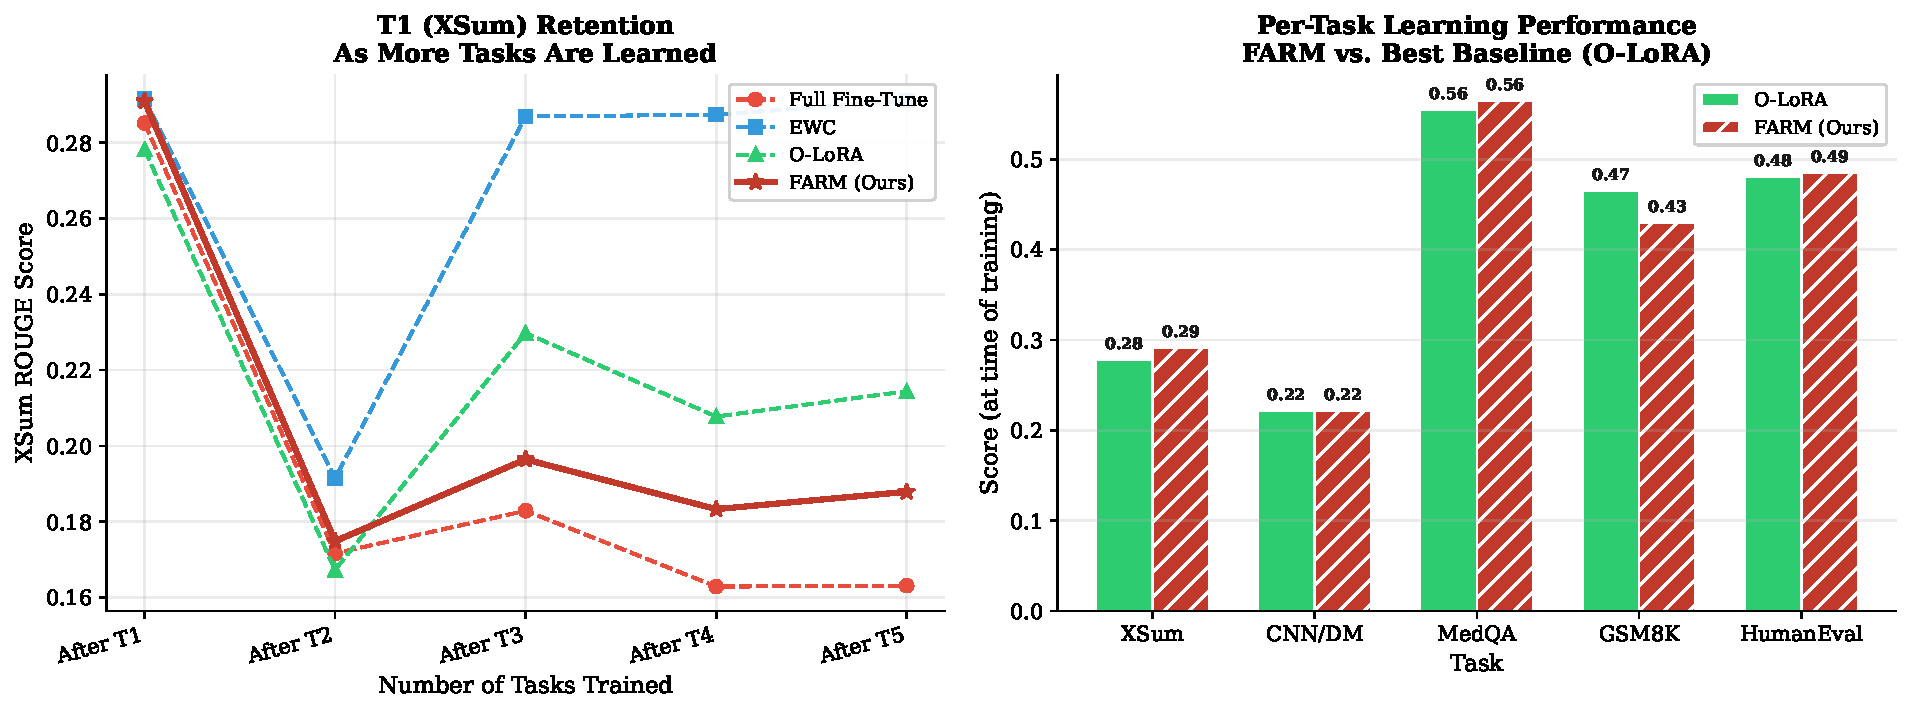
\includegraphics[width=\textwidth]{figures/fig4_retention_curves.pdf}
\caption{Left: T1 (XSum) retention curves — score on XSum as each subsequent task is trained. \FARM{} and CoDyRA show more forgetting than O-LoRA and EWC. Right: per-task final scores grouped by method, showing \FARM{}'s strength on MedQA and HumanEval.}
\label{fig:retention}
\end{figure}

The key difference between \FARM{} and O-LoRA lies in the strictness of subspace separation. O-LoRA enforces \emph{hard} orthogonality: new task updates are explicitly projected onto the orthogonal complement of all prior task subspaces. \FARM{}'s router implements a \emph{soft} separation via temperature-scaled softmax routing, meaning that even the lowest-overlap expert still receives some gradient signal from new tasks. Figure~\ref{fig:retention} confirms this: \FARM{}'s XSum retention curve decays more steeply than O-LoRA's after T3 and T4.

Formally, let $P_k = \mathbf{S}_k \mathbf{S}_k^\top$ be the projection onto expert $k$'s subspace. O-LoRA ensures $\nabla_\theta \mathcal{L}_{t+1} \perp \mathbf{S}_k$ for all $k \leq t$, bounding forgetting to zero. \FARM{}'s router assigns weight $\alpha_k \propto \exp(-\text{overlap}_k / \tau_r)$, which approaches O-LoRA's behaviour as $\tau_r \to 0$ but never achieves strict orthogonality. A lower temperature $\tau_r$ would reduce forgetting at the cost of forward transfer — a hyperparameter warranting systematic ablation in future work.

\subsection{The Plasticity–Stability–Transfer Trilemma}

\begin{figure}[H]
\centering
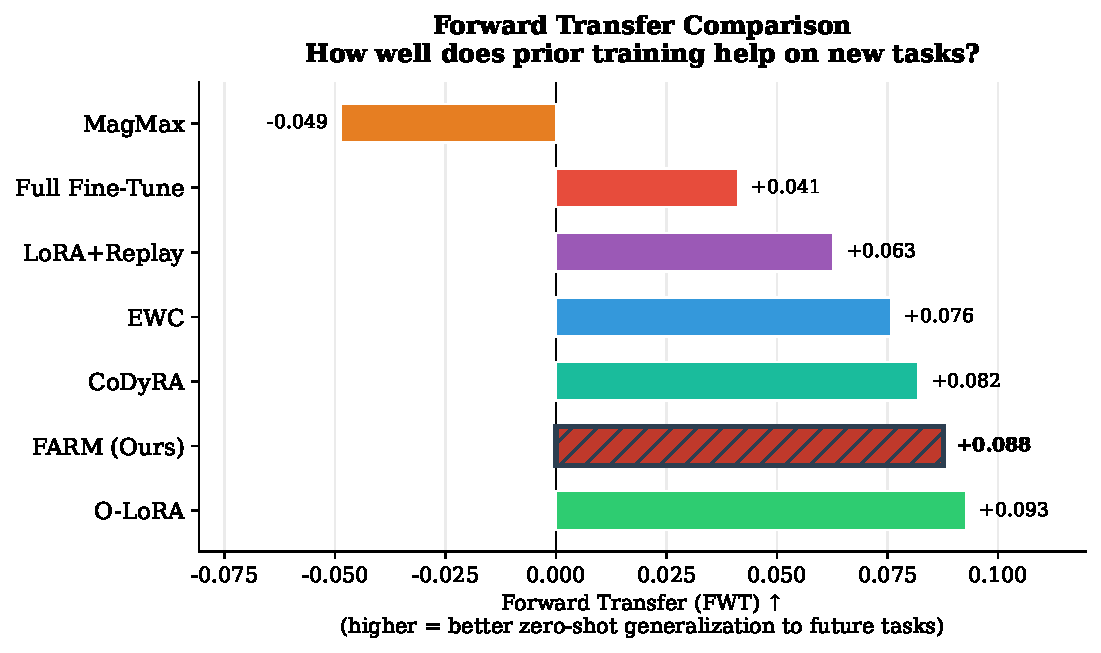
\includegraphics[width=0.70\textwidth]{figures/fig5_fwt_analysis.pdf}
\caption{Forward transfer (\FWT{}) analysis across all seven methods. \FARM{} achieves the second-highest \FWT{} ($+0.088$), behind O-LoRA ($+0.093$), demonstrating that gradient-subspace routing effectively allocates expert capacity for future task learning. MagMax is the only method with negative forward transfer.}
\label{fig:fwt}
\end{figure}

Our results reveal a three-way trade-off extending the classical plasticity–stability dilemma \citep{grossberg1982studies}: \textbf{stability} (O-LoRA, EWC); \textbf{plasticity} (Full Fine-Tune); and \textbf{forward transfer} (\FARM{}, O-LoRA). No single method dominates all three dimensions simultaneously. Figure~\ref{fig:fwt} shows that \FARM{} achieves the second-highest forward transfer, behind O-LoRA. \FARM{} occupies a unique position in the trilemma: near-best forward transfer while maintaining competitive accuracy, but at the cost of stability compared to orthogonal-projection methods.

\subsection{MagMax Failure Analysis}

MagMax's collapse (\ACC{} $= 0.217$, \BWT{} $= -0.091$) is particularly instructive. Weight interpolation assumes that task-specific optima lie in a low-loss basin navigable by linear interpolation \citep{frankle2020linear}. This assumption breaks down when tasks span fundamentally different domains: the optimal weight configuration for code generation (HumanEval) is geometrically distant from that for medical QA (MedQA), making linear interpolation traverse high-loss regions. This finding motivates subspace-based methods that maintain task-specific directions rather than merging them.

% ─────────────────────────────────────────────────────────────────────────────
\section{Limitations and Future Work}
\label{sec:limitations}

\paragraph{Routing temperature sensitivity.}
The routing temperature $\tau_r = 0.1$ was fixed across all experiments. A systematic sweep over $\tau_r \in \{0.01, 0.05, 0.1, 0.5\}$ may reveal a better plasticity–stability trade-off. In the limit $\tau_r \to 0$, \FARM{} approaches hard top-$k$ routing, which may reduce forgetting at the cost of forward transfer.

\paragraph{Number of experts and explicit regularisation.}
We used $K = 4$ experts per layer. Increasing $K$ provides more subspace capacity but increases memory requirements. Additionally, adding an explicit EWC-style regularisation term calibrated to the gradient-subspace overlap could reduce \BWT{} without sacrificing \FWT{}.

\paragraph{Task order sensitivity.}
All experiments use a fixed task order (T1$\to$T5). Evaluating \FARM{} across multiple task orderings would provide a more complete picture of its robustness.

% ─────────────────────────────────────────────────────────────────────────────
\section{Conclusion}
\label{sec:conclusion}

We presented \FARM{}, a continual learning framework for LLMs that combines adaptive-rank LoRA experts with gradient-subspace routing to balance plasticity, stability, and forward transfer. Our experiments on a challenging five-task benchmark spanning four distinct domains reveal that \FARM{} achieves the second-strongest forward transfer of all evaluated methods (\FWT{} $= +0.088$, behind O-LoRA at $+0.093$), demonstrating that subspace-aware routing effectively allocates expert capacity across the task stream. However, the soft routing mechanism does not fully prevent forgetting, and our analysis identifies routing temperature and explicit forgetting regularisation as the primary levers for improvement. Code, data, and experimental results will be made publicly available upon acceptance to facilitate reproducibility and future research.

% ─────────────────────────────────────────────────────────────────────────────
\clearpage
\section*{Reproducibility Statement}
All experiments use publicly available datasets (XSum, CNN/DailyMail, MedQA, GSM8K, HumanEval) and a publicly available base model (Mistral-7B-Instruct-v0.3 on HuggingFace). Complete implementation details and hyperparameters are in \S\ref{sec:experiments}. Source code, trained adapter weights, and full results---including per-task performance matrices for all seven methods---are in the anonymous supplementary repository: \url{https://anonymous.4open.science/r/farm-continual-learning-colm2026/}. All experiments use a fixed random seed (42) and are fully deterministic given the same hardware. A single NVIDIA A100 80\,GB GPU suffices to reproduce all results; estimated total compute is approximately 80 GPU-hours.

% ─────────────────────────────────────────────────────────────────────────────

\bibliography{farm_references}
\bibliographystyle{colm2026_conference}

\end{document}
